% (c) 2014 Daniele Zambelli - daniele.zambelli@gmail.com
% 
% Tutti i grafici per il capitolo relativo agli iperreali
%

%-------------------------------------------------
% al corso di NSA Verona 2020

%%%%%%%%%%%%%%%%%%%%%%%%%%%%%%%%%%%%%%%%%%%%%%%%%%%%%%%%%%%%%%%%%%%%
%
%        Corso Analisi Non Standard - Verona 2020
%
%                      Gruppo NSA-Verona
%
%                  Dai razionali agli iperreali
%
%                            grafici
%
% This work may be distributed and/or modified under the
% conditions of the Creative Commons BY-SA
%
% The Current Maintainer of this work is 
% Daniele Zambelli - daniele.zambelli@gmail.com
%
% Copyright 2020-24 Daniele Zambelli
%%%%%%%%%%%%%%%%%%%%%%%%%%%%%%%%%%%%%%%%%%%%%%%%%%%%%%%%%%%%%%%%%%%%
\begin{comment}
\input{\lbr preambolo}


\begin{scope} % red + green = yellow
	\clip (90:1.5) circle(2cm);
	\draw [draw=none, fill=yellow] (-30:1.5) circle (2cm);
\end{scope} % blue + red = magenta
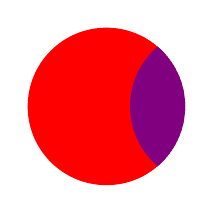
\begin{tikzpicture}[
  radius=10mm,
]
  \begin{scope}
    \clip (0, 0) circle;
    \fill[red] (0, 0) circle;
    \fill[red!50!blue, overlay] (13mm, 0) circle;
  \end{scope}
\end{tikzpicture}

\end{comment}

% \newcommand{\rettarazionali}{% Retta con alcuni esempi di numeri
%   \disegno[20]{
%     \foreach \xi/\si in {-2/\(\dots\), -1, 0, 1, 2, 3/\(\dots\)}
%       {\filldraw (\xi, 0) circle (1pt) [blue]
%                           node [below, blue] {\si};}
%     \foreach \num/\den/\xl/\yl in {3/2/0.4/-.50, 5/3/0.6/-.52, 
%                                   7/4/0.8/-.54, 9/5/1.0/-.56, 
%                                   11/6/1.2/-.58, 13/7/1.4/-.60, 
%                                   15/8/1.6/-.62, 17/9/1.8/-.64, 
%                                   19/10/2.0/-.66, 21/11/2.2/-.68}
%       {\draw (\num / \den, 0) circle (1pt) [blue];
%        \draw [angle 45 -, blue] (\num / \den, 0) to [out=270, in=90]
%         (\xl, \yl) node [below] {\footnotesize \(\frac{\num}{\den}\)};}
%     \asse{-2}{3}{0}{}
%   }
% }

\newcommand{\microa}[4]{
  \def \px{#1}
  \def \py{#2}
  \def \dy{#3}
  \def \punti{#4}
    \microscopio{(\px, \py)}{1.}{85}{275}{3}{(\px+3.7, \py+5.3)}
                {\footnotesize \(\times 10\)}
    \draw (\px-2.8-.3, \py+\dy) -- (\px+2.5+.3, \py+\dy);
    \foreach \p/\l in \punti {
      \draw (\p, \py+\dy+.1) -- (\p, \py+\dy-.1)
        node [left, rotate=90] {\footnotesize \(\l\)};}
}

\newcommand{\ingrandimenti}{% 
  \disegno[4]{
    \assecontrattini{-4}{+4}{0}{}
    \foreach \x in {-3, ..., +3}
      {\draw (\x, 0) -- (\x, -.22) node [below] {\footnotesize \(\x\)};} 
    \microa{0}{0}{4}{\px-2.8/-0.2, \px-1.8/-0.1, \px-0.8/0, 
                     \px+0.2/+0.1, \px+1.2/+0.2, \px+2.2/+0.3}
    \microa{-.8}{4}{4}{\px-2.8/-0.02, \px-1.8/-0.01, \px-0.8/0, 
                       \px+0.2/+0.01, \px+1.2/+0.02, \px+2.2/+0.03}
    \microa{-1.6}{8}{4}{\px-2.8/-0.002, \px-1.8/-0.001, \px-0.8/0, 
                        \px+0.2/+0.001, \px+1.2/+0.002, \px+2.2/+0.003}
  }
}

\newcommand{\internob}{
  \draw (\xasseda, \yasse) -- (\xassea, \yasse);
  \begin{scope}
  	\clip \centro circle(\raggio mm);
    \fill [brown!70!black] \recta rectangle \rectb;
  \end{scope}
  \draw (\puntoa, \yasse) -- (\puntoa, \yasse -.2) node [below] 
        {\labela};
  \draw (\puntob, \yasse) -- (\puntob,\yasse -.2) node [below] 
        {\labelb};
}

\newcommand{\misura}[1]{% 
  % misura di un segmento.
  \def \posrettdue{#1}
  \def \fri{-.8}
  \def \frf{-.05}
  \def \pos{7.23}
%   \disegno[4]{
  \disegno[10]{
    \assecontrattini{-1}{9}{0}{}
%     \draw [-{Stealth[length=2mm, open, round]}, black] (-2, 0) -- (10, 0); 
    \begin{scope}
      \draw (0, 0) node [below] {\(0\)}; 
      \draw (1, 0) node [below] {\(1\)}; 
      \draw (7, 0) node [below=.1] {\(m\)}; 
      \draw (8, 0) node [below] {\(m+1\)}; 
%       \draw (\pos-1, \fri) node [below left] {\(m\)}--(\pos-.23, \frf); 
%       \draw (\pos+1, \fri) node [below right=-.3] {\(m+1\)}--
%                  (\pos+.77, \frf); 
    \end{scope}
    \fill [brown!70!black] (0, 0.005) rectangle (\pos, 0.15)
    node [midway, above] {\(l\)};
    \microscopio{(0, .05)}{.5}{85}{265}{1.5}{(2, 3)} {\(\times n\)}
    \microscopio{(\pos, .05)}{.5}{85}{275}{1.5}{(9, 3)} {\(\times n\)}
    \def \xasseda{-1.33}
    \def \xassea{1.67}
    \def \yasse{2.}
    \def \centro{(.175, 2.04)}
    \def \raggio{14.92}
    \def \recta{(-0, 2.005)}
    \def \rectb{(2.4, 3.)}
    \def \puntoa{0}
    \def \labela{\(0\)}
    \def \puntob{1}
    \def \labelb{\(\dfrac{1}{n}\)}
    \internob
    \def \xasseda{5.65}
    \def \xassea{8.65}
    \def \centro{(7.13, 2.05)}
    \def \recta{(5, 2.005)}
    \def \rectb{(\posrettdue, 3.)}
    \def \puntoa{6.7}
    \def \labela{\(\dfrac{s}{n}\)}
    \def \puntob{7.7}
    \def \labelb{\(\dfrac{s+1}{n}\)}
    \internob
  }
}

\newcommand{\internoc}{
  \draw (\xasseda, \yasse) -- (\xassea, \yasse);
  \begin{scope}
  	\clip \centro circle(\raggio mm);
    \fill [brown!70!black] \recta rectangle \rectb;
  \end{scope}
  \draw (\puntoa, \yasse) -- (\puntoa, \yasse -.2) 
        node [below=-.22, xshift=\shifta mm] 
        {\labela};
  \draw (\puntob, \yasse) -- (\puntob,\yasse -.2) 
        node [below=-.22, xshift=\shiftb mm] 
        {\labelb};
}

\newcommand{\approssimazioni}{% 
  % misura di un segmento.
%   \def \fri{-.8}
%   \def \frf{-.05}
  \def \pos{1.4142}
  \disegno[4]{
    \draw [-{Stealth[length=2mm, open, round]}, black] (-1.3, 0) -- (3, 0);
    \foreach \x in {-1, ..., 2}
      {\draw (\x, 0) -- (\x, -.22) node [below] {\footnotesize \(\x\)};} 
    \fill [brown!70!black] (0, 0.015) rectangle (\pos, 0.2);
    \microscopio{(\pos, .05)}{1.5}{85}{275}{2}{(4, 4)}
                {\footnotesize \(\times 10\)}
    \def \xasseda{-.6}
    \def \xassea{3.35}
    \def \yasse{3.2}
    \def \centro{(1.37, 3.535)}
    \def \raggio{7.93}
    \def \recta{(-.8, 3.215)}
    \def \rectb{(1.4142, 5)}
    \def \puntoa{1.3}
    \def \shifta {-1}
    \def \labela{\footnotesize \(1.4\)}
    \def \puntob{2.3}
    \def \shiftb {+1}
    \def \labelb{\footnotesize \(1.5\)}
    \internoc
    \microscopio{(\pos, \yasse)}{1.5}{85}{275}{2}{(4, 7.2)}
                {\footnotesize \(\times 10\)}
%     \def \xasseda{-.6}
%     \def \xassea{3.35}
    \def \yasse{6.4}
    \def \centro{(1.37, 6.735)}
%     \def \raggio{7.93}
    \def \recta{(-.8, 6.415)}
    \def \rectb{(1.4142, 9)}
    \def \puntoa{1}
    \def \shifta {-1.5}
    \def \labela{\footnotesize \(1.41\)}
    \def \puntob{2}
    \def \shiftb {+1.5}
    \def \labelb{\footnotesize \(1.42\)}
    \internoc
    \microscopio{(\pos, \yasse)}{1.5}{85}{275}{2}{(4, 10.4)}
                {\footnotesize \(\times 10\)}
%     \def \xasseda{-.6}
%     \def \xassea{3.35}
    \def \yasse{9.6}
    \def \centro{(1.37, 9.935)}
%     \def \raggio{7.93}
    \def \recta{(-.8, 9.615)}
    \def \rectb{(1.4142, 12)}
    \def \puntoa{1.2}
    \def \shifta {-2.5}
    \def \labela{\footnotesize \(1.414\)}
    \def \puntob{2.2}
    \def \shiftb {+2.5}
    \def \labelb{\footnotesize \(1.415\)}
    \internoc
  }
}

\newcommand{\poligoniregolari}{

% Radius of regular polygons
  \def \R{1.3}

  \disegno[10]{
    % Indicate the boundary of the regular polygons
%     \draw [thin,black!20] circle (\R) ;
%     \fill[black!20] circle (2pt);
    \draw [very thick, blue!50!black] (0:\R) -- (120:\R) 
          node [midway, above right=-.15] {\(u\)} -- 
          (240:\R) -- cycle;
    \draw [very thick, orange!50!black] (0:\R) -- 
          (180:\R*0.5) node [midway, below left=-.1] {\(h\)};
    \begin{scope}[xshift=30mm*\R]
    \draw [very thick, blue!50!black] (0:\R) -- (90:\R) 
          node [midway, above right=-.15] {\(u\)} -- 
          (180:\R) -- (270:\R) -- cycle;
    \draw [very thick, orange!50!black] (0:\R) -- 
          (180:\R) node [midway, below] {\(d\)};
    \end{scope}
    \begin{scope}[xshift=60mm*\R]
    \draw [very thick, blue!50!black] (0:\R) -- (72:\R) 
          node [midway, above right=-.15] {\(u\)} -- 
          (144:\R) -- (216:\R) -- (288:\R) -- cycle;
    \draw [very thick, orange!50!black] (0:\R) -- 
          (144:\R) node [midway, below left=-.1] {\(d\)};
    \end{scope}
  }
}

\newcommand{\frecciav}[4]{% Freccia verticale.
  % Esempio di chiamata:
  % \frecciav{-.25}{-.04}{-.12}{}
  \def \posx{#1}
  \def \ymi{#2}
  \def \yma{#3}
  \def \lab{#4}
%   \draw [-{Stealth[length=2mm, round]}] (\posx, \yma) -- (\posx, \ymi);
  \draw [-{Straight Barb[length=4pt,width=2pt, round]}] 
         (\posx, \yma) -- (\posx, \ymi);
  \node [above] at (\posx, \yma) {\lab};
}

\newcommand{\rettaappross}{% 
  % Alcuni punti del segmento 0-1.
  \asse{-8}{+8}{0}{};
%   \foreach \x in {.02, .04, ..., .3}{
  \foreach \x in {.1, .2, .4, .8, 1.6, 3.2}{
    \draw (-\x, 0) arc [start angle=0, end angle=+20, radius=.8];
    \draw (\x, 0) arc [start angle=180, end angle=160, radius=.8];}
}

\newcommand{\unoconnome}{% 
  % Sezione con elementi separatori di cui due con nome
\disegno{
  \rettaappross
  \frecciav{-2.5}{-.4}{-1.2}{}
  \frecciav{2.5}{-0.4}{-1.2}{}
  \node at(-.8, .4)[above] {\(q_1\)};
  \node at(1.6, .4) [above] {\(q_2\)};
  \draw [<->] (-2.4, -1.2) -- node [below] {\(\frac{1}{n}\)} (2.4, -1.2);
  \microscopio{(0, .2)}{1.}{89}{-90}{2}{(2, 5.)}{\(\times \infty\)}
  \draw (-2.0, 3.1) -- (+2.0, 3.1);
  \draw (0, 3.3) -- (0, 3.1);
    \node at (0, 3.1) [below] {\(a\)};
  }
}

\newcommand{\molticonnome}{% 
  % Sezione con elementi separatori di cui due con nome
\disegno{
  \rettaappross
  \frecciav{-2.5}{-.4}{-1.2}{}
  \frecciav{2.5}{-0.4}{-1.2}{}
  \node at(-.8, .4)[above] {\(q_1\)};
  \node at(1.6, .4) [above] {\(q_2\)};
  \draw [<->] (-2.4, -1.2) -- node [below] {\(\frac{1}{n}\)} (2.4, -1.2);
  \microscopio{(0, .2)}{1.}{89}{-90}{2}{(2, 5.)}{\(\times \infty\)}
  \draw (-2.0, 3.1) -- (+2.0, 3.1);
  \foreach \x in {-1.2, -.6, ..., 1.2}
    \draw (\x, 3.3) -- (\x, 3.1);
    \node at (-.6, 3.1) [below] {\(\alpha\)};
    \node at (.6, 3.1) [below] {\(\beta\)};
  }
}

% \newcommand{\internomonade}{
%   \draw (\xasseda, \yasse) -- (\xassea, \yasse);
%   \draw (\puntoa, \yasse) -- (\puntoa, \yasse -.2) 
%         node [below=-.22, xshift=-2.3mm] {\labela};
%   \draw (\puntob, \yasse) -- (\puntob, \yasse -.2) 
%         node [below=-.04] {\labelb};
%   \draw (\puntoc, \yasse) -- (\puntoc, \yasse -.2) 
%         node [below=-.22, xshift=+0mm] {\labelc};
% }
% 
% \newcommand{\monade}{% 
%   % misura di un segmento.
%   \disegno[4]{
%     \draw [-{Stealth[length=2mm, open, round]}, black] (-3, 0) -- (3, 0);
%     \draw (0, 0) -- (0, -.22) node [below] {\footnotesize \(a\)};
%     \microscopio{(0, .05)}{1.5}{85}{275}{2}{(2.2, 5.3)}
%                 {\footnotesize \(\times \infty\)}
%     \def \xasseda{-2.0}
%     \def \xassea{+1.93}
%     \def \yasse{3.2}
%     \def \puntoa{-1.5}
%     \def \labela{}
%     \def \puntob{0}
%     \def \labelb{\footnotesize \(a\)}
%     \def \puntoc{+1.5}
%     \def \labelc{\footnotesize \(a+\delta\)}
%     \internomonade
%   }
% }

% fine estratto corso
%-------------------------------------

\newcommand{\microscopioa}{% Microscopio per vedenodere 5,004.
    \disegno{
    \assecontrattini{-1.3}{+6.3}{0}{x}
    \draw (0, 0) [below] node{0} (1, 0) [below] node{1}
          (5, 0) [below] node{5};
    \microscopio{(5, 0)}{2.5}{90}{-50}{3.5}{(5.5, 8.5)}{\(\times 10^3\)}
    \segmentocontrattini{-.3}{+6}{5.5}{1}
    \draw (2.8, 5.5) [left] node [rotate=90] {5,000} 
          (3.8, 5.5) [left] node [rotate=90] {5,001}
          (0.8, 5.5) [left] node [rotate=90] {4,998};
    }
}

\newcommand{\microscopiob}{% Microscopio per vedere -3,000002.
    \disegno{
    \assecontrattini{-4.3}{+3.3}{0}{x}
    \draw (0, 0) [below] node{0} (1, 0) [below] node{1}
          (-3, 0) [below] node{-3};
    \microscopio{(-3, 0)}{2.5}{70}{-115}{3.5}{(3.5, 9)}{}
    \segmentocontrattini{-3.9}{+2.5}{5.5}{1}
    }
}

\newcommand{\microscopioc}{% Microscopio per NON vedere 2 - 3 \epsilon.
    \disegno{
    \assecontrattini{-1.3}{+6.3}{0}{x}
    \draw (0, 0) [below] node{0} (1, 0) [below] node{1}
          (2, 0) [below] node{2};
    \microscopio{(2, 0)}{2.5}{60}{-100}{3.5}{(7.5, 8.5)}{\(\times 10^{27}\)}
    \draw[very thin] (3.8, 6-.1) -- (3.8, 6+0.2);
    \draw [-] (0.4, 6) -- (7.3, 6);
    \draw [-{Stealth[length=2mm, round]}] 
      (3, 5) node [below] {\(2-\epsilon\)} -- (3.8, 6);
    \draw [-{Stealth[length=2mm, round]}] 
      (5, 5) node [below] {\(2\)} -- (3.8, 6);
    }
}

\newcommand{\microscopiod}{% Microscopio per vedere 2 - 3 \epsilon.
    \disegno{
    \assecontrattini{-1.3}{+6.3}{0}{x}
    \draw (0, 0) [below] node{0} (1, 0) [below] node{1}
          (2, 0) [below] node{2};
    \microscopio{(2, 0)}{2.5}{60}{-100}{3.5}{(7.5, 8.5)}
                {\(\times \frac{1}{\epsilon}\)}
    \segmentocontrattini{.7}{7}{6}{1}
    \draw (.8, 6) [left] node [rotate=90] {\(2 - 3 \epsilon\)} 
          (2.8, 6) [left] node [rotate=90] {\(2 - \epsilon\)}
          (3.8, 6) [left] node [rotate=90] {2};
    }
}

\newcommand{\telescopioa}{% Telescopio per visualizzare 127034.
    \disegno{
    \assecontrattini{-1.3}{+6.3}{0}{x}
    \draw (0, 0) [below] node{0} (1, 0) [below] node{1};
    \draw (-1, 1) pic [rotate=0, scale=.5] {telescopio=127034};
    \microscopio{(-1, 1)}{2.5}{40}{-130}{3.5}{(7.5, 9.5)}{}
    \segmentocontrattini{0}{+6.2}{6}{1}
    \draw (1., 6) [left] node [rotate=90] {...} 
          (2., 6) [left] node [rotate=90] {127033} 
          (3., 6) [left] node [rotate=90] {127034}
          (4., 6) [left] node [rotate=90] {127035}
          (5., 6) [left] node [rotate=90] {\dots};
    }
}

\newcommand{\telescopiob}{% Telescopio per visualizzare 127034.
    \disegno{
    \assecontrattini{-1.3}{+6.3}{0}{x}
    \draw (0, 0) [below] node{0} (1, 0) [below] node{1};
    \draw (-1, 1) pic [rotate=0, scale=.5] {telescopio=\(A\)};
    \microscopio{(-1, 1)}{2.5}{40}{-130}{3.5}{(7.5, 9.5)}{}
    \segmentocontrattini{0}{+6.2}{6}{1}
    \draw (0, 6) [left] node [rotate=90] {\dots} 
          (1, 6) [left] node [rotate=90] {\(A - 1\)} 
          (2, 6) [left] node [rotate=90] {\(A ~~\quad\)}
          (3, 6) [left] node [rotate=90] {\(A + 1\)}
          (5, 6) [left] node [rotate=90] {\(A + 3\)}
          (6, 6) [left] node [rotate=90] {\dots};
    }
}

\newcommand{\grandangoloa}{% Grandangolo per vedenodere 300.
    \disegno{
    \assecontrattini{-1.3}{+6.3}{0}{x}
    \draw (0, 0) [below] node{0} (1, 0) [below] node{1};
    \grandangolo{(0, 0)}{2.5}{90}{-126}{3.5}{(5.5, 8.5)}{\(\div 100\)}
    \segmentocontrattini{-1.1}{+5.2}{6}{1}
    \draw (1.9, 6) [left] node [rotate=90] {0} 
          (2.9, 6) [left] node [rotate=90] {100}
          (4.9, 6) [left] node [rotate=90] {300};
    }
}

\newcommand{\grandangolob}{% Grandangolo per vedenodere 300.
    \disegno{
    \assecontrattini{-1.3}{+6.3}{0}{x}
    \draw (0, 0) [below] node{0} (1, 0) [below] node{1};
    \grandangolo{(0, 0)}{2.5}{90}{-126}{3.5}{(5.5, 8.5)}{\(\div A\)}
    \segmentocontrattini{-1.1}{+5.2}{6}{1}
    \draw (1.9, 6) [left] node [rotate=90] {0} 
          (2.9, 6) [left] node [rotate=90] {\(A\)}
          (-.1, 6) [left] node [rotate=90] {\(-2 A\)};
    }
}

\newcommand{\combinazione}{% Combinazione per: \(1741,998+2\epsilon\).
    \disegnod{4}{
    \assecontrattini{-1.3}{+6.3}{0}{x}
    \draw (0, 0) [below] node{0} (1, 0) [below] node{1};
    \draw (-1, 1) pic [rotate=0, scale=.5] {telescopio=1742};
    \microscopio{(-1, 1)}{2.5}{40}{-130}{3.5}{(7.5, 9.5)}{}
    \segmentocontrattini{0}{+6.2}{6}{1}
    \draw (1., 6) [left] node [rotate=90] {\dots}
          (2., 6) [left] node [rotate=90] {1741}
          (3., 6) [left] node [rotate=90] {1742}
          (4., 6) [left] node [rotate=90] {1743}
          (5., 6) [left] node [rotate=90] {\dots};
    \microscopio{(3., 6)}{2.5}{130}{-40}{3.5}{(-5.2, 12.7)}{\(\times 1000\)}
    \segmentocontrattini{-4.5}{+1.9}{10.5}{1}
    \draw (-3.5, 10.5) [left] node [rotate=90] {\dots}
          (-2.5, 10.5) [left] node [rotate=90] {1741,998}
          (-1.5, 10.5) [left] node [rotate=90] {1741,999}
          (-0.5, 10.5) [left] node [rotate=90] {1742}
          (0.5, 10.5) [left] node [rotate=90] {\dots};
    \microscopio{(-2.5, 10.5)}{2.5}{30}{-120}{3.5}{(5, 17)}
                {\(\times \frac{1}{\epsilon}\)}
    \segmentocontrattini{-1.77}{+4.6}{15}{1}
    \draw (-0.7, 15) [right] node [rotate=90] {\dots}
          (0.3, 15) [right] node [rotate=90] {1742,998}
          (1.3, 15) [right] node [rotate=90] {\(1741,998+\epsilon\)}
          (2.3, 15) [right] node [rotate=90] {\(1741,998+2\epsilon\)}
          (3.3, 15) [right] node [rotate=90] {\dots};
    }
}

\newcommand{\espdueterzi}{% 
    % Esponenziali con basi diverse.
    \disegno{
    \rcom{-10}{+10}{-1}{10}{gray!50, very thin, step=1}
    \begin{scope}[ultra thick, color=Maroon!50!black]
      \tkzInit[xmin=-10.3,xmax=+10.3,ymin=-0.3,ymax=+10.3]
      \tkzFct[domain=-10.3:+6]{(3./2)**x}
%       \begin{scope}[color=Green!50!black]
        \tkzFct[color=Green!50!black, domain=-6:+10.3]{(2./3)**x}
%       \end{scope}
      \begin{scope}[color=Black!50!black]
        \filldraw (1, 3./2) circle (1.2pt);
        \filldraw (1, 2./3) circle (1.2pt);
      \end{scope}
%       \begin{scope}[color=Red!50!black]
        \filldraw [color=Red!50!black] (0, 1) circle (1.2pt);  
%       \end{scope}
    \end{scope}
    \begin{scope}[color=black]
      \draw (-4.1, 9.5) node{\(a < 1\)}; 
      \draw ((6.6, 9.5) node{\(a > 1\)};
    \end{scope}
    }
}

\newcommand{\logduebasi}{% 
    % Esponenziali con basi diverse.
    \disegno{
    \rcom{-1}{+10}{-10}{10}{gray!50, very thin, step=1}
    \begin{scope}[ultra thick, color=Maroon!50!black]
    \tkzInit[xmin=-1.3,xmax=+10.3,ymin=-10.3,ymax=+10.3]
    \tkzFct[domain=0:+10.3]{log(x)/log(3./2)}
    \filldraw (3./2, 1) circle (1.2pt);
    \begin{scope}[color=Green!50!black]
    \tkzFct[domain=0:+10.3]{log(x)/log(2./3)}
    \filldraw (3./2, -1) circle (1.2pt);
    \end{scope}
    \end{scope}
    \begin{scope}[color=black]
      \draw (8.5, -4.5) node{\(a < 1\)}; 
      \draw (8.5, 6.6) node{\(a > 1\)};
    \end{scope}
    }
}

% \newcommand{\logduebasi}{% 
%     % Esponenziali con basi diverse.
%     \disegno{
%     \rcom{-1}{+10}{-10}{10}{gray!50, very thin, step=1}
%     \begin{scope}[ultra thick, color=Maroon!50!black]
%     \tkzInit[xmin=-1.3,xmax=+10.3,ymin=-10.3,ymax=+10.3]
%     \tkzFct[domain=0:+10.3]{log(x)/log(3)}
%     \tkzFct[domain=0:+10.3]{log(x)/log(2)}
%     \tkzFct[domain=0:+10.3]{log(x)/log(3./2)}
%     \tkzFct[domain=0:+10.3]{log(x)/log(5./4)}
%     \foreach \pi in {(3, 1), (2, 1), (3./2, 1), (5./4, 1)}
%       \filldraw \pi circle (1.2pt);
%     \begin{scope}[color=Green!50!black]
%     \tkzFct[domain=0:+10.3]{log(x)/log(1./3)}
%     \tkzFct[domain=0:+10.3]{log(x)/log(1./2)}
%     \tkzFct[domain=0:+10.3]{log(x)/log(2./3)}
%     \tkzFct[domain=0:+10.3]{log(x)/log(4./5)}
%     \foreach \pi in {(3, -1), (2, -1), (3./2, -1), (5./4, -1)}
%       \filldraw \pi circle (1.2pt);
%     \end{scope}
%     \end{scope}
%     \begin{scope}[color=black]
%     \draw (7.5, 9.5) node{a} (9.5, 5.2) node{b} 
%           (9.5, 2.8) node{c} (9.5, 1.5) node{d}; 
%     \draw (9.5, -1.5) node{e} (9.5, -2.8) node{f} 
%           (9.5, -5.2) node{g} (7.5, -9.5) node{h};
%     \end{scope}
%     }
% }
